\documentclass[a4paper,14pt]{extarticle}

\usepackage[utf8]{inputenc}
\usepackage[T2A]{fontenc}
\usepackage[english, russian]{babel}

\usepackage[mode=buildnew]{standalone}
\usepackage{setspace}


% Различные пакеты
\usepackage{
	amssymb, amsfonts, amsmath, amsthm, physics,
	cancel, indentfirst,makecell,multirow, 
	graphicx, tikz, mathtools, float, setspace,caption,subcaption
} 

\usepackage{mathtools}

% Эта опция включает нумерацию только у тех формул,
% на которые есть ссылка в документе
\mathtoolsset{showonlyrefs=true} 

 % Цвета для гиперссылок
\definecolor{linkcolor}{HTML}{000000} % цвет ссылок
\definecolor{urlcolor}{HTML}{799B03} % цвет гиперссылок
 
\usepackage{xcolor}
\usepackage[
    unicode, 
    colorlinks, 
    urlcolor=urlcolor, 
    linkcolor=linkcolor,
    citecolor=linkcolor
]{hyperref}

% Увеличенный межстрочный интервал, французские пробелы
\linespread{1.2} 
\frenchspacing 

%%%%%%%%%%%%%%%%%%%%%%%%%%%%%%
%  Пользовательские команды  %
%%%%%%%%%%%%%%%%%%%%%%%%%%%%%%


\makeatletter
    \newcommand{\fftStar}[1]{\mathfrak{F}^*\qty[#1]}
    \newcommand{\fftNoStar}[1]{\mathfrak{F}\qty[#1]}
    \newcommand{\fft}{
                 \@ifstar
                 \fftStar%
                 \fftNoStar%
    }
\makeatother

\makeatletter
    \newcommand{\ifftNoStar}[1]{\mathfrak{F}^{-1}\qty[#1]}
    \newcommand{\ifftStar}[1]{\qty(\mathfrak{F}^{-1}\qty[#1])^*}
    \newcommand{\ifft}{
                 \@ifstar
                 \ifftStar%
                 \ifftNoStar%
    }
\makeatother

\newcommand{\mean}[1]{\langle#1\rangle}
\newcommand\ct[1]{\text{\rmfamily\upshape #1}}
\newcommand*{\const}{\ct{const}}
\renewcommand{\phi}{\varphi}
\renewcommand{\epsilon}{\varepsilon}
%\renewcommand{\sigma}{\varsigma}


\captionsetup{subrefformat=parens}

\usepackage{array}
\usepackage{pstool}


% Диагональная ячейка в таблице ( типа |a/b|)
\newcolumntype{x}[1]{>{\centering\arraybackslash}p{#1}}
\newcommand\diag[4]{%
  \multicolumn{1}{p{#2}|}{\hskip-\tabcolsep
  $\vcenter{\begin{tikzpicture}[baseline=0,anchor=south west,inner sep=#1]
      \path[use as bounding box] (0,0) rectangle (#2+2\tabcolsep,\baselineskip);
      \node[minimum width={#2+2\tabcolsep},minimum height=\baselineskip+\extrarowheight] (box) {};
      \draw (box.north west) -- (box.south east);
      \draw (box.south west) -- (box.north west);
      \node[anchor=south west] at (box.south west) {\footnotesize#3};
      \node[anchor=north east] at (box.north east) {\footnotesize#4};
 \end{tikzpicture}}$\hskip-\tabcolsep}}

%%%%%%%%%%%%%%%%%%%%%%%%%%%%%
%  Геометрия и колонтитулы  %
%%%%%%%%%%%%%%%%%%%%%%%%%%%%%


\usepackage{geometry}
\geometry       
    {
        left            =   2cm,
        right           =   2cm,
        top             =   2.5cm,
        bottom          =   2.5cm,
        bindingoffset   =   0cm
    }

% Настройка содержания, точки после нумераций
\usepackage{tocloft}
\addto\captionsrussian{\renewcommand{\contentsname}{Оглавление}}
\renewcommand{\cftsecleader}{
	\cftdotfill{\cftdotsep}}
% \renewcommand{\thesection}{
	% \arabic{section}.}
% \renewcommand{\thesubsection}{
	% \arabic{section}.\arabic{subsection}.}
% \renewcommand{\thesubsubsection}{
	% \arabic{section}.\arabic{subsection}.\arabic{subsubsection}.}     
\usepackage[explicit]{titlesec}

% Колонтитулы
\usepackage{fancyhdr} 
	\pagestyle{plain} 
	\fancyhead{} 
	\fancyhead[R]{} 
	\fancyhead[L]{} 
	\fancyfoot{} 
	\fancyfoot[C]{\thepage} 

\title{Компьютерные технологии}
\author{Понур К.А. 
    \thanks{исходники (*.py, *.tex):
    https://github.com/kannab98/computer-technologies}
}
\begin{document}
\maketitle

\paragraph{Задание 20} Используя метод  прямоугольников  и  метод  выборочного  среднего, вычислите моменты инерции тела сложного объема с неоднородной плотностью при его вращении вокруг трех  перпендикулярных  осей. Оцените точность  и  время  вычислений  в  обоих  случаях в зависимости от схемы интегрирования.

\tableofcontents
\section{Постановка задачи}
%Момент инерции тела относительно произвольной оси, проходящей через центр масс и имеющей направление, заданное единичным вектором s → = ‖ s x , s y , s z ‖ T , | s → | = 1 {\displaystyle {\vec {s}}=\left\Vert s_{x},s_{y},s_{z}\right\Vert ^{T},\left\vert {\vec {s}}\right\vert =1} {\displaystyle {\vec {s}}=\left\Vert s_{x},s_{y},s_{z}\right\Vert ^{T},\left\vert {\vec {s}}\right\vert =1}, можно представить в виде квадратичной (билинейной) формы:

%Согласно \cite{MomOfInertia} момент инерции вокруг произвольной оси вычисляется

Пусть плотность исследуемого тела задается в декартовой системе координат 
некоторой функцией $\rho(x,y,z)$

\subsection{Метод прямоугольников}%
\label{sub:metod_priamougol_nikov}

Наиболее простой метод численного интегрирования заключается в аппроксимации
подынтегральной функции $f(x)$ многочленом нулевой степени на каждом
элементарном отрезке. Для $n$ элементарных отрезков подобная составная
квадратурная формула на линейной координатной сетке с шагом
$h=\frac{b-a}{n}$ примет вид
\begin{equation}
    \label{eq:}
    \int\limits_{a}^{b} f(x) \dd x \approx h\frac{f(x_0)}{2} +
    h\frac{f(x_n)}{2} + h\sum\limits_{i=1}^{n-1} f(x_i) 
\end{equation}

Погрешность  вычисления интеграла на $i$-ом элементарном отрезке в таком случае определяется формулой
\begin{equation}
    \label{eq:}
    \epsilon(f) = \dv[2]{f(\xi)}{\xi} \cdot \frac{h^2}{24}(x_i - x_{i-1}),
\end{equation}
где $\xi_i = \frac{x_{i-1} + x_i}{2}$ -- середина рассматриваемого элементарного
отрезка.

\subsection{Метод Монте-Карло}%
\label{sub:metod_monte_karlo}

Сущность метода Монте-Карло состоит в следующем: необходимо найти значение $a$
некоторой изучаемой величины. Для этого выбирают величину  $x$, математическое
ожидание которой равно  $a$, т.е.
 \begin{equation}
    \label{eq:}
    M(X) = a
\end{equation}

На практике это означает проведение $n$ независимых испытаний и вычисление
среднего значения величины $x$ по полученному ансамблю данных
\begin{equation}
    \label{eq:}
    \mean{x} = \frac{1}{n} \sum\limits_{i=1}^{n} x_i.
\end{equation}

Величину $\mean{x}$ принимают в качестве оценки  $a^*$ исходной величины  $a$.
Пусть теперь $J$ значение интеграла на интервале  $[a,b]$ функции $f(x)$
 \begin{equation}
    \label{eq:}
    J = \int\limits_{a}^{b}  f(x) \dd x
\end{equation}

Тогда
\begin{equation}
    \label{eq:}
    \mean{f(x)} \approx \frac{1}{n} \sum\limits_{i=1}^{n} f(x_i)
\end{equation}
И сам интеграл
\begin{equation}
    \label{eq:}
    \mean{J} \approx \frac{b-a}{n} \sum\limits_{i=1}^{n} f(x_i)
\end{equation}



\subsection{Adaptive quadrature}%
\label{sub:adaptive_quadrature}


Для сравнения с предыдущими методами интегрирования применим более общий метод
численного интегрирования Adaptive Quadrature, используемый в библиотеке SciPy
\cite{SciPy} на основе Фортран-библиотеке численного интегрирования QUADPACK
\cite{QuadPack}.

В основе метода лежит интерполяции искомой функции $f(x)$ детерменированными
полиномами на определенных интервалах, например, полиномами Чебышева или
полиномами Лежандра. 


\section{Реализации на языке Python}

В качестве тела достаточно сложного объема был выбран тороид, располагаемый в
начале координат и задаваемый параметрическим уравнением в сферической системе
координат
\begin{equation}
    \label{eq:tor}
    \begin{cases}
        x(\phi, \psi) = (R + r\cos \psi) \cos \phi \\
        y(\phi, \psi) = (R + r\cos \psi) \sin \phi \\
        z(\phi, \psi) = r\sin \psi
    \end{cases}
    \phi \in [0, 2\pi), \psi \in [-\pi, \pi),
\end{equation}
где $\phi$ -- азимутальный угол в плоскости  $xy$,  $\psi$ -- угол элевации,
отсчитываемый от оси $z$. На рис. \ref{fig:tor}
\begin{figure}[h]
    \centering
    \begin{subfigure}{0.49\linewidth}
        \centering
        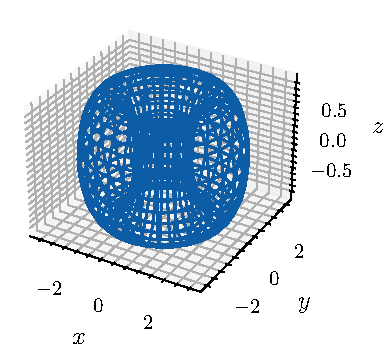
\includegraphics[width=1\linewidth]{figs_20/tor}
    \end{subfigure}
    \begin{subfigure}{0.49\linewidth}
        \centering
        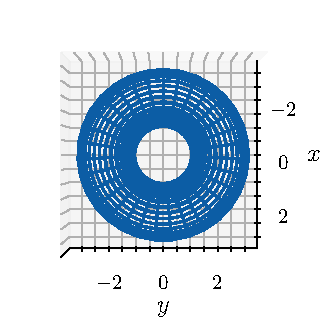
\includegraphics[width=1\linewidth]{figs_20/tor-top}
    \end{subfigure}
    \caption{Тороид с внутренним радиусом $r=1$  и внешним радиусом  $R=2$}
    \label{fig:tor}
\end{figure}




\end{document}
